\documentclass[12pt,a4paper]{article}

% Core formatting packages
\usepackage[a4paper, margin=0.75in]{geometry}
\usepackage{graphicx}
\usepackage{amsmath, amssymb}
\usepackage{setspace}
\usepackage{parskip}
\usepackage{enumitem}
\usepackage{xcolor}
\usepackage{mdframed}
\usepackage{listings}
\usepackage{tcolorbox}
\usepackage{hyperref}

\tcbuselibrary{skins, breakable}

% Colors matching reference layout
\definecolor{tasktitleblue}{RGB}{0, 0, 180}
\definecolor{taskboxbg}{RGB}{245, 247, 255}
\definecolor{darkboxbg}{RGB}{30, 30, 30}
\definecolor{darkboxheader}{RGB}{50, 50, 50}

% Syntax highlighting setup for Python source code
\definecolor{codegreen}{rgb}{0,0.6,0}
\definecolor{codegray}{rgb}{0.5,0.5,0.5}
\definecolor{codepurple}{rgb}{0.58,0,0.82}
\definecolor{backcolour}{rgb}{0.96,0.96,0.96}

\lstdefinestyle{pystyle}{
    backgroundcolor=\color{backcolour},   
    commentstyle=\color{codegreen},
    keywordstyle=\color{magenta},
    numberstyle=\tiny\color{codegray},
    stringstyle=\color{codepurple},
    basicstyle=\ttfamily\footnotesize,
    breakatwhitespace=false,         
    breaklines=true,                 
    captionpos=b,                    
    keepspaces=true,                 
    numbers=left,                    
    numbersep=5pt,                  
    showspaces=false,                
    showstringspaces=false,
    showtabs=false,                  
    tabsize=4
}
\lstset{style=pystyle}

% Custom Task Box Environment (Blue Framed Header)
\newtcolorbox{taskbox}[1]{
    colframe=tasktitleblue,
    colback=taskboxbg,
    coltitle=white,
    fonttitle=\bfseries\large,
    title=#1,
    arc=4pt,
    outer arc=4pt,
    boxrule=1.5pt,
    left=10pt, right=10pt, top=8pt, bottom=8pt
}

% Custom Sample Input Box
\newtcolorbox{sampleinputbox}[1][Sample Input]{
    colframe=darkboxheader,
    colback=backcolour,
    coltitle=white,
    fonttitle=\bfseries,
    title=#1,
    arc=3pt,
    boxrule=1pt,
    left=8pt, right=8pt, top=6pt, bottom=6pt
}

% Custom Sample Output Box
\newtcolorbox{sampleoutputbox}[1][Sample Output]{
    colframe=darkboxheader,
    colback=darkboxbg,
    coltitle=white,
    fonttitle=\bfseries,
    title=#1,
    arc=3pt,
    boxrule=1pt,
    left=8pt, right=8pt, top=6pt, bottom=6pt
}

\setlength{\parindent}{0pt}
\onehalfspacing

\begin{document}

% ==========================================
% PAGE 1: TITLE HEADER & LAB CHECKLIST
% ==========================================
\begin{center}
    {\large \textbf{Department of Computer Science}} \\
    {\large \textbf{Human-Computer Interaction (HCI) \& Computer Graphics (CG)}} \\[12pt]
    
    {\Huge \textbf{Assignment 3}} \\[6pt]
    {\Large \textbf{(LAB 1: Display Density Metrics \& Image Array Mechanics in NumPy)}} \\[14pt]
    
    \rule{\textwidth}{0.8pt} \\[10pt]
    
    \begin{tabular}{ll}
        \textbf{Student Name:} Partab Rai & \textbf{Roll Number:} 2k24/CSE/117 \\
        \textbf{Program:} Computer Science (Part III P.E) & \textbf{Submission Date:} September 11, 2026
    \end{tabular}
    
    \rule{\textwidth}{0.8pt}
\end{center}

\vspace{1.5em}

\section*{Lab Deliverables Checklist}
\begin{mdframed}[backgroundcolor=gray!5, linecolor=tasktitleblue, linewidth=1pt, roundcorner=4pt]
    \begin{itemize}[label=$\checkmark$, leftmargin=2em]
        \item \textbf{Task 1: Display Pixel Density (PPI/DPI) Calculator}
        \begin{itemize}[label=$\bullet$, leftmargin=1.5em]
            \item Interactive CLI script for PPI calculation \& aspect ratio reduction.
            \item Automated density classification rules (Low, Medium, High).
            \item Console outputs \& execution screenshots attached.
        \end{itemize}
        
        \vspace{0.3em}
        \item \textbf{Task 2: Environment Setup \& Synthetic Image Matrix Creation}
        \begin{itemize}[label=$\bullet$, leftmargin=1.5em]
            \item $300 \times 400 \times 3$ uint8 3D NumPy matrix constructed from scratch.
            \item Spatial quadrant slicing for pure Red, Green, Blue, and White colors.
            \item Array properties ($\text{shape}, \text{dtype}, \text{size}, \text{nbytes}$) logged.
        \end{itemize}
        
        \vspace{0.3em}
        \item \textbf{Task 3: Channel Slicing \& Isolation}
        \begin{itemize}[label=$\bullet$, leftmargin=1.5em]
            \item 2D channel intensity grid extraction using Axis 2 slicing.
            \item Single-channel color isolations rendered alongside grayscale views.
            \item $2 \times 3$ Matplotlib subplot visualization rendered and attached.
        \end{itemize}
        
        \vspace{0.3em}
        \item \textbf{Task 4: Spatial Downsampling \& Pixelation via Striding}
        \begin{itemize}[label=$\bullet$, leftmargin=1.5em]
            \item Matrix downsampling via step-slicing (\texttt{img[::N, ::N, :]}) for $N=8$.
            \item Re-expansion using \texttt{np.repeat()} to visualize blocky pixelation.
            \item Spatial dimension drop and 98.44\% memory savings calculated.
        \end{itemize}
        
        \vspace{0.3em}
        \item \textbf{Short Answer Theory Question}
        \begin{itemize}[label=$\bullet$, leftmargin=1.5em]
            \item Mathematical explanation for 33.33\% RAM increase in RGBA vs RGB.
        \end{itemize}
    \end{itemize}
\end{mdframed}

\newpage

% ==========================================
% PAGE 2: TASK 1
% ==========================================
\begin{taskbox}{Task 1: Display Pixel Density (PPI/DPI) Calculator}
\textbf{Objective:} Write a Python script that calculates screen parameters and classifies display density based on physical screen attributes.

\textbf{Requirements:}
\begin{enumerate}[leftmargin=*]
    \item Prompt the user to input horizontal pixels ($W_{\text{px}}$), vertical pixels ($H_{\text{px}}$), and physical screen diagonal ($D_{\text{inches}}$).
    \item Calculate and display:
    \begin{itemize}[leftmargin=*]
        \item Total pixel count ($W_{\text{px}} \times H_{\text{px}}$).
        \item Simplified aspect ratio ($W : H$) using the greatest common divisor (\texttt{math.gcd}).
        \item Screen DPI/PPI rounded to two decimal places.
    \end{itemize}
    \item Classify the display density into one of the following categories:
    \begin{itemize}[leftmargin=*]
        \item $\text{DPI} < 100$: \textbf{Low Density} (Standard Monitor)
        \item $100 \le \text{DPI} \le 200$: \textbf{Medium Density} (HD Display)
        \item $\text{DPI} > 200$: \textbf{High Density} (Retina / Mobile)
    \end{itemize}
\end{enumerate}
\end{taskbox}

\vspace{0.3em}
\textbf{Sample Execution:}

\begin{sampleinputbox}
Enter horizontal resolution (pixels): 1920\\
Enter vertical resolution (pixels): 1080\\
Enter physical diagonal size (inches): 24
\end{sampleinputbox}

\begin{sampleoutputbox}
\color{white}\ttfamily
--- DISPLAY METRICS ANALYSIS ---\\
Total Pixel Count : 2,073,600 pixels\\
Aspect Ratio      : 16:9\\
Calculated DPI    : 91.79 DPI\\
Density Category  : Low Density (Standard Monitor)
\end{sampleoutputbox}

\vspace{0.4em}
\subsection*{Source Code (Task 1)}
\begin{lstlisting}[language=Python]
import math

Wpx = int(input("Enter horizontal resolution (pixels): "))
Hpx = int(input("Enter vertical resolution (pixels): "))
Dinches = float(input("Enter physical diagonal size (inches): "))

total_pixels = Wpx * Hpx
gcd = math.gcd(Wpx, Hpx)
aspect_width = Wpx // gcd
aspect_height = Hpx // gcd
dpi = ((Wpx**2 + Hpx**2) ** 0.5) / Dinches

if dpi < 100:
    density_category = "Low Density (Standard Monitor)"
elif dpi <= 200:
    density_category = "Medium Density (HD Display)"
else:
    density_category = "High Density (Retina / Mobile)"

print("--- DISPLAY METRICS ANALYSIS ---")
print(f"Total Pixel Count : {total_pixels:,} pixels")
print(f"Aspect Ratio      : {aspect_width}:{aspect_height}")
print(f"Calculated DPI    : {dpi:.2f} DPI")
print(f"Density Category  : {density_category}")
\end{lstlisting}

\vspace{0.4em}
\subsection*{Actual Task 1 Output Screenshots}
\begin{figure}[h!]
    \centering
    \begin{minipage}{0.49\textwidth}
        \centering
        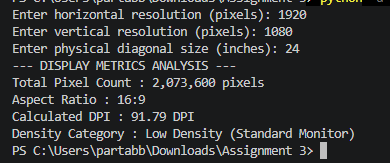
\includegraphics[width=\textwidth]{outputs/task1_desktop.png}
        \caption{Desktop Test Screenshot}
    \end{minipage}
    \hfill
    \begin{minipage}{0.49\textwidth}
        \centering
        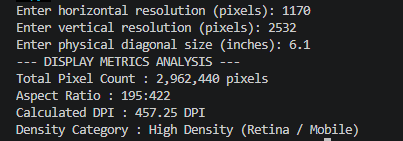
\includegraphics[width=\textwidth]{outputs/task1_mobile.png}
        \caption{Mobile Test Screenshot}
    \end{minipage}
\end{figure}

\newpage

% ==========================================
% PAGE 3: TASK 2
% ==========================================
\begin{taskbox}{Task 2: Environment Setup \& Synthetic Image Matrix Creation}
\textbf{Objective:} Install Python graphics packages and construct a 3D image matrix from scratch.

\textbf{Requirements:}
\begin{enumerate}[leftmargin=*]
    \item Install required packages: \texttt{pip install numpy pillow matplotlib}.
    \item Create a synthetic $300 \times 400 \times 3$ image array initialized with zeros using \texttt{np.zeros()} with data type \texttt{np.uint8}.
    \item Fill the four quadrants using spatial array slicing \texttt{[row\_start:row\_end, col\_start:col\_end]}:
    \begin{itemize}[leftmargin=*]
        \item Top-Left: Pure Red \texttt{[255, 0, 0]}, Top-Right: Pure Green \texttt{[0, 255, 0]}
        \item Bottom-Left: Pure Blue \texttt{[0, 0, 255]}, Bottom-Right: White \texttt{[255, 255, 255]}
    \end{itemize}
    \item Print matrix properties: \texttt{.shape}, \texttt{.dtype}, \texttt{.size}, and \texttt{.nbytes}.
\end{enumerate}
\end{taskbox}

\vspace{0.3em}
\textbf{Sample Execution:}

\begin{sampleoutputbox}
\color{white}\ttfamily
--- SYNTHETIC MATRIX METRICS ---\\
Array Shape (H, W, C) : (300, 400, 3)\\
Data Type            : uint8\\
Total Elements       : 360,000 values\\
Memory Footprint     : 360,000 bytes (351.56 KB)
\end{sampleoutputbox}

\vspace{0.4em}
\subsection*{Source Code (Task 2)}
\begin{lstlisting}[language=Python]
import numpy as np
import matplotlib.pyplot as plt

image = np.zeros((300, 400, 3), dtype=np.uint8)
image[:150, :200] = [255, 0, 0]      # Top-Left: Red
image[:150, 200:] = [0, 255, 0]      # Top-Right: Green
image[150:, :200] = [0, 0, 255]      # Bottom-Left: Blue
image[150:, 200:] = [255, 255, 255]  # Bottom-Right: White

print("--- SYNTHETIC MATRIX METRICS ---")
print(f"Array Shape (H, W, C) : {image.shape}")
print(f"Data Type            : {image.dtype}")
print(f"Total Elements       : {image.size:,} values")
print(f"Memory Footprint     : {image.nbytes:,} bytes ({image.nbytes / 1024:.2f} KB)")

plt.imshow(image)
plt.axis('off')
plt.savefig('outputs/task2_synthetic.png', bbox_inches='tight', pad_inches=0)
plt.show()
\end{lstlisting}

\vspace{0.4em}
\subsection*{Actual Task 2 Output Image}
\begin{figure}[h!]
    \centering
    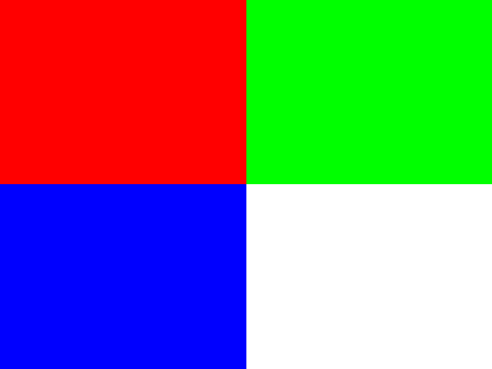
\includegraphics[width=0.75\textwidth]{outputs/task2_synthetic.png}
    \caption{Task 2: Generated Synthetic Quadrant Matrix (\texttt{task2\_synthetic.png})}
\end{figure}

\newpage

% ==========================================
% PAGE 4: TASK 3
% ==========================================
\begin{taskbox}{Task 3: Channel Slicing \& Isolation}
\textbf{Objective:} Load an image, extract individual 2D channel intensity grids, and isolate single-channel color views in a $2 \times 3$ layout.

\textbf{Requirements:}
\begin{enumerate}[leftmargin=*]
    \item Load an input image (\texttt{sample.jpg}) into a NumPy array.
    \item Extract 2D intensity grids for Red, Green, and Blue channels using Axis 2 slicing.
    \item Construct three separate 3D color arrays where only one channel is active.
    \item Render in a $2 \times 3$ subplot layout (Top Row: Color Isolations, Bottom Row: Grayscale Intensities).
\end{enumerate}
\end{taskbox}

\vspace{0.3em}
\textbf{Sample Execution:}

\begin{sampleoutputbox}
\color{white}\ttfamily
--- CHANNEL EXTRACTION SUMMARY ---\\
Original Image Shape   : (1080, 1920, 3)\\
Red Channel 2D Shape   : (1080, 1920) | Mean Intensity: 176.51\\
Green Channel 2D Shape : (1080, 1920) | Mean Intensity: 220.18\\
Blue Channel 2D Shape  : (1080, 1920) | Mean Intensity: 235.71\\
Display Window         : Matplotlib 2x3 Subplot Grid Rendered.
\end{sampleoutputbox}

\vspace{0.4em}
\subsection*{Source Code (Task 3)}
\begin{lstlisting}[language=Python]
import numpy as np
from PIL import Image
import matplotlib.pyplot as plt

image = np.array(Image.open("sample.jpg").convert("RGB"))

red_channel = image[:, :, 0]
green_channel = image[:, :, 1]
blue_channel = image[:, :, 2]

red_only = np.zeros_like(image); red_only[:, :, 0] = red_channel
green_only = np.zeros_like(image); green_only[:, :, 1] = green_channel
blue_only = np.zeros_like(image); blue_only[:, :, 2] = blue_channel

fig, axes = plt.subplots(2, 3, figsize=(12, 8))
axes[0, 0].imshow(red_only); axes[0, 0].set_title("Red-Only")
axes[0, 1].imshow(green_only); axes[0, 1].set_title("Green-Only")
axes[0, 2].imshow(blue_only); axes[0, 2].set_title("Blue-Only")

axes[1, 0].imshow(red_channel, cmap="gray"); axes[1, 0].set_title("Red Intensity")
axes[1, 1].imshow(green_channel, cmap="gray"); axes[1, 1].set_title("Green Intensity")
axes[1, 2].imshow(blue_channel, cmap="gray"); axes[1, 2].set_title("Blue Intensity")

for ax in axes.flat:
    ax.axis("off")

plt.tight_layout()
plt.savefig("outputs/task3_subplots.png", bbox_inches="tight")
plt.show()
\end{lstlisting}

\vspace{0.4em}
\subsection*{Actual Task 3 Output Image}
\begin{figure}[h!]
    \centering
    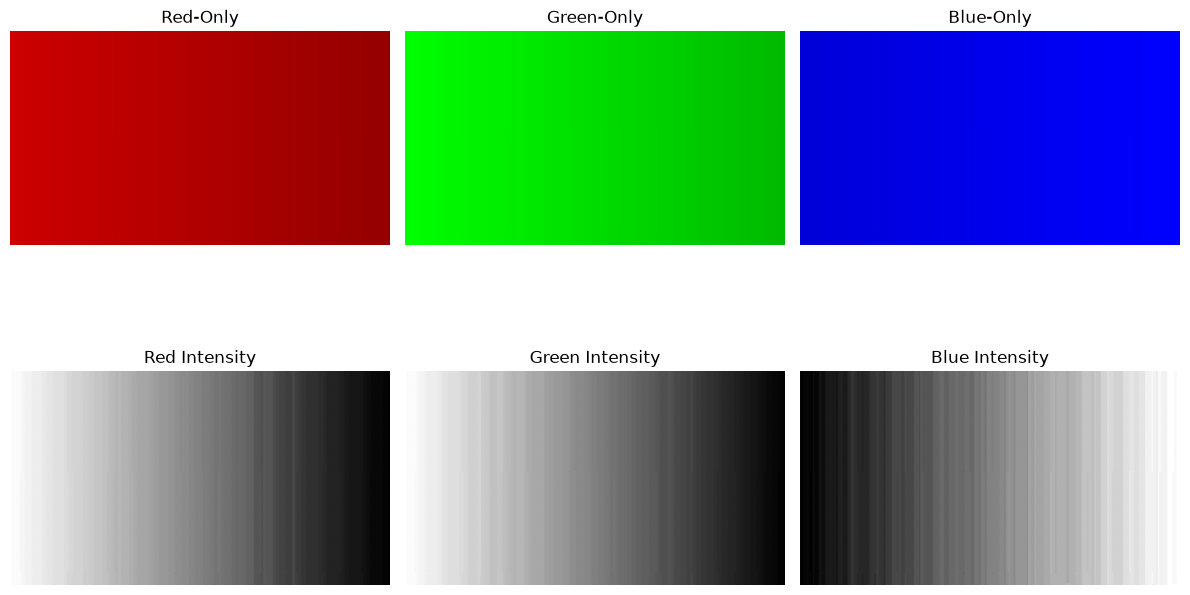
\includegraphics[width=0.98\textwidth]{outputs/task3_subplots.png}
    \caption{Task 3: Matplotlib 2x3 Subplot Channel Grid (\texttt{task3\_subplots.png})}
\end{figure}

\newpage

% ==========================================
% PAGE 5: TASK 4
% ==========================================
\begin{taskbox}{Task 4: Spatial Downsampling \& Pixelation via Striding}
\textbf{Objective:} Perform spatial downsampling directly in NumPy using slice steps and analyze memory reduction.

\textbf{Requirements:}
\begin{enumerate}[leftmargin=*]
    \item Downsample an input image matrix by taking every $N$-th pixel using NumPy striding (\texttt{img[::N, ::N, :]}) for $N=8$.
    \item Re-expand downsampled array back to original dimensions using \texttt{np.repeat()} to observe blocky pixelation.
    \item Compute spatial dimension reduction percentage and memory footprint savings.
\end{enumerate}
\end{taskbox}

\vspace{0.3em}
\textbf{Sample Execution:}

\begin{sampleoutputbox}
\color{white}\ttfamily
--- DOWNSAMPLING ANALYSIS (N = 8) ---\\
Original Shape    : (1080, 1920, 3) | Memory: 6,220,800 bytes\\
Downsampled Shape : (135, 240, 3) | Memory: 97,200 bytes\\
Re-expanded Shape : (1080, 1920, 3) | Visual: Blocky Pixelation\\
Dimension Reduction: 87.50\% reduction per axis\\
Memory Savings    : 98.44\% data reduction
\end{sampleoutputbox}

\vspace{0.4em}
\subsection*{Source Code (Task 4)}
\begin{lstlisting}[language=Python]
import numpy as np
from PIL import Image
import matplotlib.pyplot as plt

image = np.array(Image.open("sample.jpg").convert("RGB"))
N = 8

downsampled = image[::N, ::N, :]
reexpanded = np.repeat(np.repeat(downsampled, N, axis=0), N, axis=1)
reexpanded = reexpanded[:image.shape[0], :image.shape[1], :]

fig, axes = plt.subplots(1, 2, figsize=(12, 6))
axes[0].imshow(image)
axes[0].set_title(f"Original Image\nShape: {image.shape}")
axes[0].axis('off')

axes[1].imshow(reexpanded)
axes[1].set_title(f"Re-expanded Pixelated Image (N={N})\nShape: {reexpanded.shape}")
axes[1].axis('off')

plt.tight_layout()
plt.savefig('outputs/task4_downsampled.png', bbox_inches='tight')
plt.show()
\end{lstlisting}

\vspace{0.4em}
\subsection*{Actual Task 4 Output Image}
\begin{figure}[h!]
    \centering
    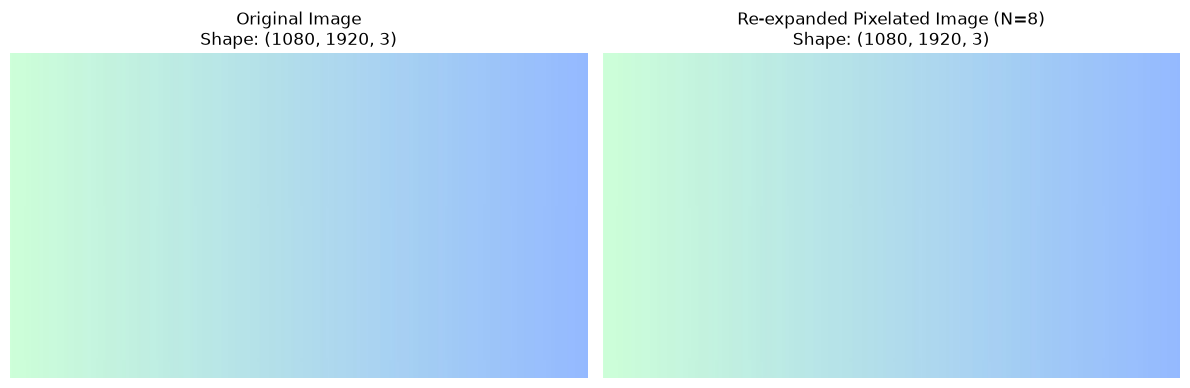
\includegraphics[width=0.98\textwidth]{outputs/task4_downsampled.png}
    \caption{Task 4: Spatial Downsampling \& Pixelation Comparison (\texttt{task4\_downsampled.png})}
\end{figure}

\vspace{70pt}

% ==========================================
% PAGE 6: SHORT ANSWER QUESTION
% ==========================================
\section*{Short Answer Theory Question}

\textbf {Why does adding an Alpha channel (RGBA) increase an image array's memory consumption by 33\% compared to standard RGB?}

\vspace{1em}
Standard RGB images store 3 color channels ($C = 3$) per pixel corresponding to Red, Green, and Blue. Adding an Alpha channel for transparency increases the channel dimension to 4 ($C = 4$). 

Because memory footprint scales linearly with total array elements ($H \times W \times C$), adding 1 additional channel to 3 channels yields a memory increase factor calculated as:
$$\frac{4 - 3}{3} = \frac{1}{3} \approx 33.33\%$$

Therefore, an RGBA image array uses exactly $33.33\%$ more memory in RAM than an RGB array of identical height and width dimensions.

\end{document}